\lecture{6. My Covenant They Broke}{06}

%------------------------------------------------------------------------------
\section{Introduction}
% this to put in this one:
% There is NO separation between church and personal life.
%--------------------------------------
\begin{frame}
\frametitle{A covenant is a contract}
\begin{columns}[T]
\begin{column}{0.5\textwidth}
	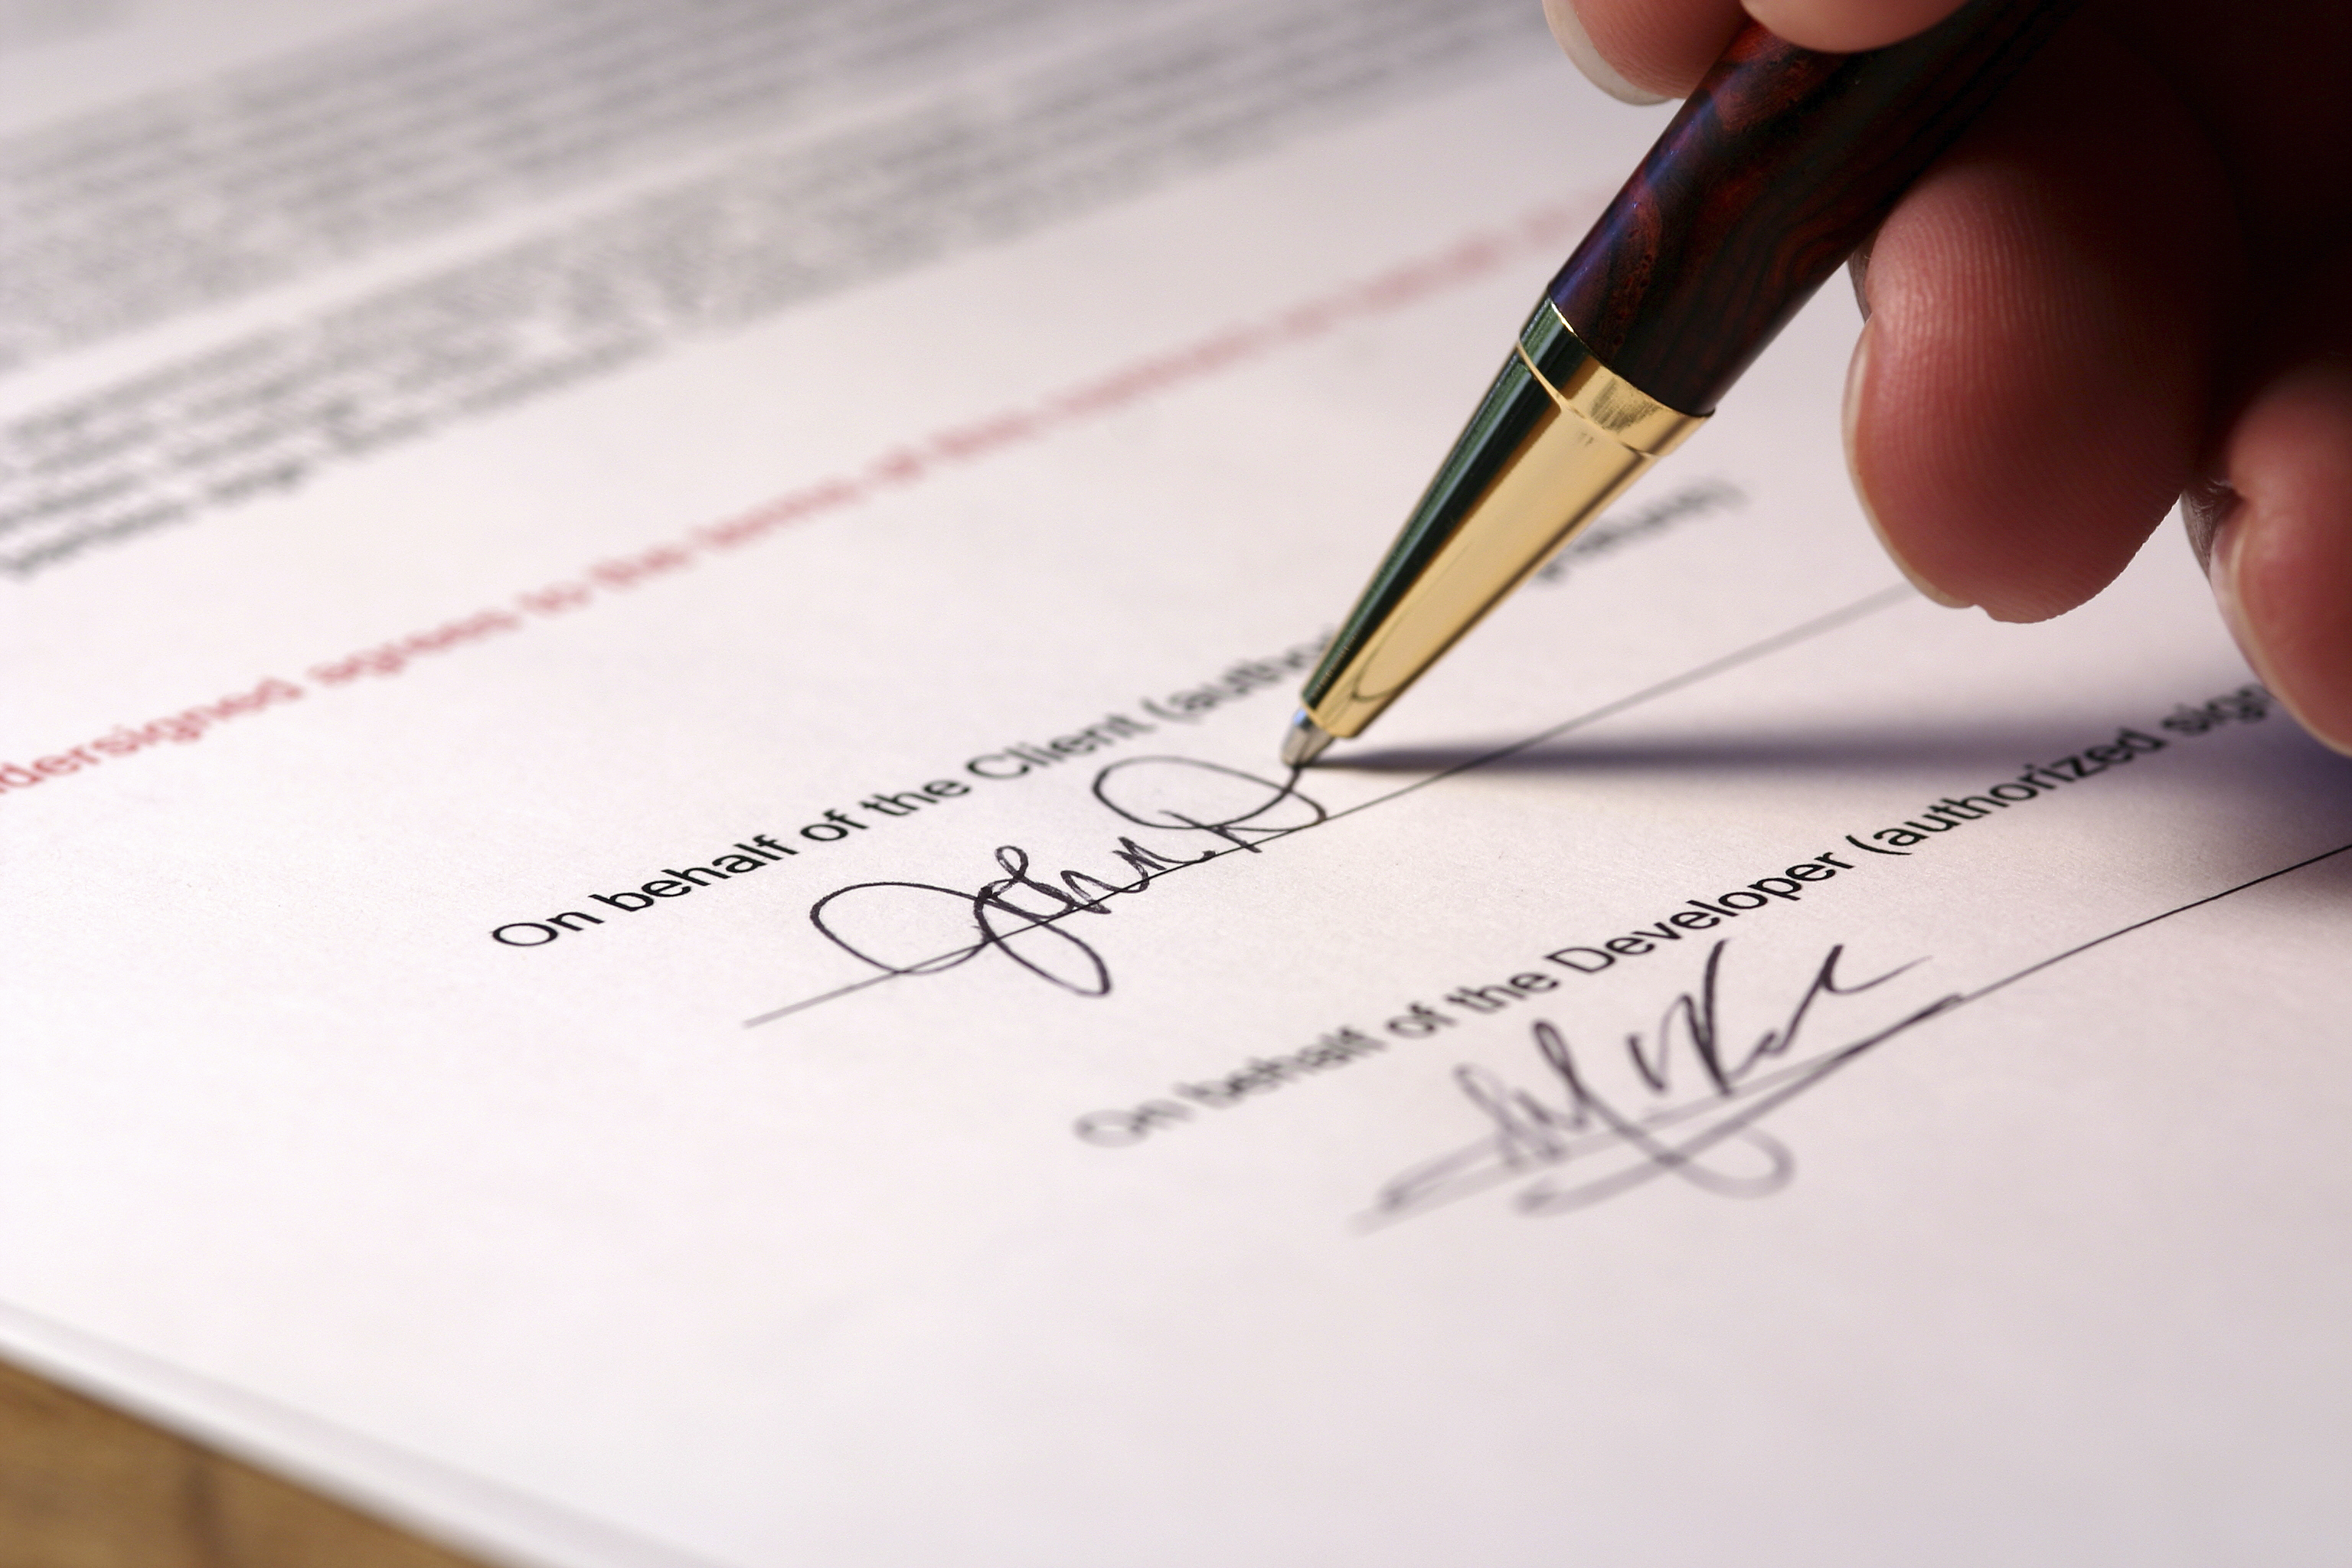
\includegraphics[width=\textwidth]{figures/contract.jpg}
\end{column}
\begin{column}{0.5\textwidth}
	Covenants can have\ldots
	\begin{itemize}
	\item requirements
	\item collateral
	\item signatures
	\item payments
	\item dates of effect
	\item etc.
	\end{itemize}
\end{column}
\end{columns}

\note{09:30}
\note[item]{Today, we're talking about how the Israelites rejected God's covenant}
\note[item]{Someone brought up a few weeks ago that a covenant is much more serious than a contract, and that's certainly true when it comes to covenants dealing with our eternal soul.}
\note[item]{However, Christians of the denominational world also make a big (false) distinction between covenants and contracts}
\note[item]{The difference, they say, is that in a covenant, one part is guaranteeing to hold up their end of the covenant even if the other party doesn't.}
\note[item]{They use this to say that even if Israel was unfaithful, God is still going to restore them physically in the millennial kingdom.}
\note[item]{They'd also note that since God has made a New Covenant, He will save the chosen regardless of how they behave}
\note[item]{We're going to study today that that's clearly not the case.}
\end{frame}

%--------------------------------------
\begin{frame}{God wants a relationship with people}
\framesubtitle{Jeremiah 31:31-34}
	\keyversehiglight{my covenant that they broke}
	
\note{09:34}
\note[item]{In the last lesson, we talked about the love that God showed to the children of Israel, and to us, like the love a husband has for His wife.}
\note[item]{Unfortunately, Israel, in general, rejected God's love}
\note[item]{Serving God, as we have discussed, is always voluntary.}
\note[item]{But, there will be consequences for unfaithfulness.}
\end{frame}

%--------------------------------------
\begin{goals}
\goal Summarize how Israel rejected God's love under the Old Covenant
\goal Examine the consequences of rejecting God's love for Israel and for
us
\goal Develop a plan to prevent falling away from God

\note{09:35}
\note[item]{We'll be considering 3 different passages today}
\note[item]{Lev. 26, one of many passages in the Old Law that lists the blessings for following God and the consequences for disobedience}
\note[item]{Heb. 3, where the writer warns Christians against following the rebellious example of the Israelites.}
\note[item]{Rom. 9:30-33, in which Paul says that Israel did not achieve righteousness from the Law because they lacked faith.}
\note[item]{For each passage we'll consider, in what ways Israel rejected God and the consequences they suffered because of that reject}
\note[item]{Finally, we'll try to learn from their bad example and think about how to prevent rejecting God's love.}
\end{goals}

%------------------------------------------------------------------------------
\section{Israel rejected God}

%--------------------------------------
\begin{frame}{Israel hardened their hearts}
\framesubtitle{Heb. 3:1-19}

	\begin{itemize}
		\item Israel rebelled against God in the wilderness (7-9,16-20)
		\item They worshiped idols
		\item They complained
		\item They did not trust God to take care of them
	\end{itemize}

\note{09:37}
\note[item]{The writer of Hebrews has been discussing how Christ is superior to the Moses.}
\note[item]{And, he's warning Christians not to reject Jesus like the children of Israel rejected God in the wilderness.}
\note[item]{Read 7-9, 16-20}
\note[item]{It's instructive to think about, what the Israelites did to reject God in the wilderness}
\note[item]{We immediately think about the golden calf, and their complaining every time they had to struggle a bit}
\note[item]{But, the incident that's specifically referred to in Hebrews is their lack of faith at the spies report when they were about to enter the land of Canaan.}
\end{frame}

%--------------------------------------
\begin{frame}{Faithfulness according to God}
\framesubtitle{Lev. 26:1-45}

	\begin{itemize}
		\item No Idols
		\item Keep the Sabbath
		\item Reverence sanctuary
	\end{itemize}

\note{09:37}
\note[item]{They seemed to get the last two, but the first one, not so much.}
\end{frame}

%--------------------------------------
\begin{frame}{Israel didn't have faith}
\framesubtitle{Rom. 9:30-33}

	\begin{itemize}
		\item Tried to obey the Law, but without faith
		\item Instead, tried to rely only on works
		\item Stumbled over Jesus.
		\item Describes well the Pharisees of Jesus' day
	\end{itemize}

\note{09:40}
\end{frame}

%------------------------------------------------------------------------------
\section{Israel suffered consequences}

%--------------------------------------
\begin{frame}{They shall not enter my rest}
\framesubtitle{Heb 3:1-19}
\begin{itemize}
	\item The wilderness was a test, which they failed
	\item So, that generation couldn't enter the promised land
	\item Their bodies fell in the wilderness
\end{itemize}

\note{09:45}
\end{frame}

%--------------------------------------
\begin{frame}{Suffering in the promised land}
\framesubtitle{Lev. 26:1-45}
\begin{itemize}
	\item Physical diseases (16)
	\item Lose to enemies(17)
    \item Poor yields (20)
    \item Kill you children and livestock (22)
    \item Starving (26,29)
    \item Lose the land (32-39)
    \item But God will bring them back (45)
\end{itemize}

\note{09:50}
\end{frame}

%--------------------------------------
\begin{frame}{Eternally Lost}
\framesubtitle{Rom. 9:30-33}
\begin{itemize}
	\item The Israelites, in general, didn't accept Jesus
	\item He was their only hope for salvation
\end{itemize}

\note{09:55}
\end{frame}

%------------------------------------------------------------------------------
\section{Avoid rejecting God}

%--------------------------------------
\begin{frame}{Do what's right}
\framesubtitle{Lev. 26:1-45}
\begin{itemize}
	\item Follow God's Law
	\item Minimize your consequences
	\item Be sensitive to change when you do have consequences.
\end{itemize}

\note{10:00}
\end{frame}

%--------------------------------------
\begin{frame}{Pursue righteousness with Faith}
\framesubtitle{Rom. 9:30-33}
\begin{itemize}
	\item Don't rely on your own righteousness
	\item Think about meeting the Lord
\end{itemize}

\note{10:05}
\end{frame}

%--------------------------------------
\begin{frame}{Don't be deceived by sin}
\framesubtitle{Heb. 3:1-19}
\begin{itemize}
	\item Hold fast to your confidence
	\item Exhort one another
    \item Don't be hardened
    \item Trust that God will take care of you
\end{itemize}

\note{10:10}
\end{frame}
%------------------------------------------------------------------------------
\section{Review}

\begin{frame}{My covenant they broke}
	\begin{itemize}
		\item Israel rejected God's love under the Old Covenant by \ldots
		\begin{itemize}
			\item not trusting God to take care of them to the promised land
			\item Worshiping idols while in the promised land
			\item Trying to rely only on works, but lacking faith
		\end{itemize}
		\item So they suffered the consequences \ldots
		\begin{itemize}
			\item The Exodus generation died in the wilderness
			\item Their descendants lost the promised land
			\item He was their only hope for salvation
		\end{itemize}
		\item Don't fall into their example \ldots
		\begin{itemize}
			\item Change when you face consequences.
			\item Pursue righteousness with faith.
			\item Trust that God will take care of you.
		\end{itemize}
	\end{itemize}
		
\note{10:12}
\end{frame}